\section{The three modules of STEPSS}

STEPSS includes three modules:
\begin{itemize}
\item {\bf PFC} (for Power Flow Computation) performs a power flow computation in order to determine the initial operating point of a dynamic simulation;
\item {\bf RAMSES} (for RApid Multithreaded Simulation of Electric power Systems) simulates the dynamic evolution of the power system in response to disturbances/actions specified by the user;
\item {\bf CODEGEN} (for CODE GENerator) translates a model described by the user in a text file into its equivalent in FORTRAN 2003 language. The latter has to be compiled and linked to a user-defined executable version RAMSES.
\end{itemize}

\begin{figure}[h!]
\centering
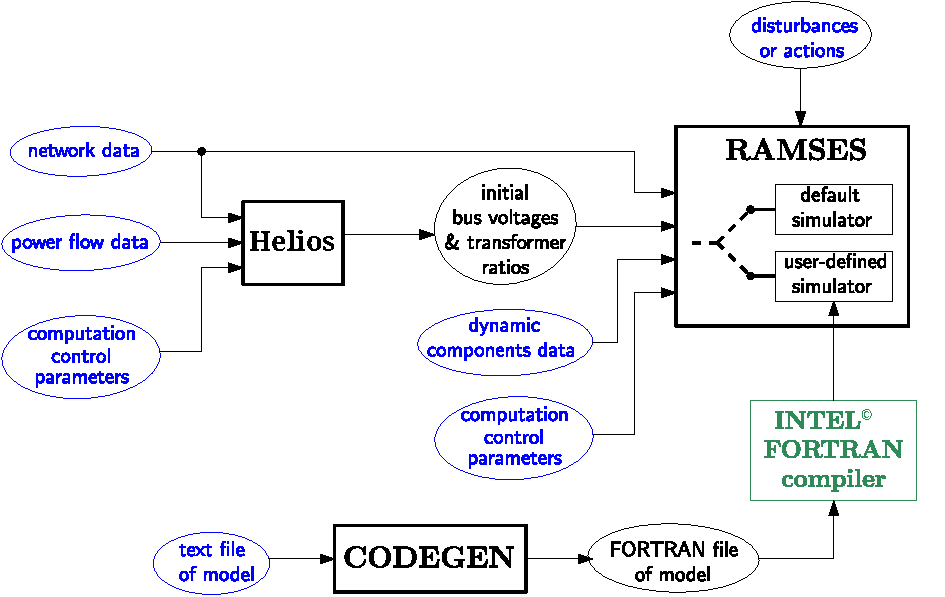
\includegraphics[scale=1.0]{over-general.pdf}
\caption{STEPSS: Overview of modules and data files. The files shown in blue are provided by the user, those in black are produced internally. The Intel$^{\copyright}$ FORTRAN compiler is not part of STEPSS}\label{fig-over-general}
\end{figure}

The three modules, their relationships and their input/ouput data files are shown graphically in Fig.~\ref{fig-over-general}.

Note that each of the three modules can be used separately. Here are examples of such uses:
\begin{itemize}
\item PFC alone: a power flow computation is run to inspect the power system state and/or save the corresponding power flow solution for use by RAMSES;
\item PFC alone: a sequence of power flow computations is performed until obtaining the desired power system state. The corresponding power flow solution is saved for use by RAMSES;
\item RAMSES alone: with the initial power flow solution produced by PFC, several dynamic simulations are run starting from that initial state, i.e. without invoking PFC each time;
\item CODEGEN alone: a model is built and saved for future incorporation in a user-defined version of RAMSES.
\end{itemize}

%--------------------------------------------------------------------------------------------------
\section{PFC module}

The power flow computation resorts to the well-known Newton(-Raphson) method. Polar coordinates are used.

As shown in Fig.~\ref{fig-over-general}, the input information consists of:
\begin{itemize}
\item network data relative to buses, lines, transformers, etc.
\item power flow data specified at PV, PQ and slack buses, respectively
\item PFC control parameters. These are settings such as: tolerances on final power mismatches, thresholds to enforce reactive power limits of generators, etc. These are optional data; if they are not provided, default values (listed in this documentation) are used.
\end{itemize}

Optionally PFC also adjusts the ratios of some transformers, with the objective:
\begin{itemize}
\item for an in-phase transformer: to bring the voltage magnitude at a bus inside a specified deadband
\item for a phase-shifting transformer: to bring the active power flow in a network branch inside a specified deadband.
\end{itemize}

PFC produces an output file including:
\begin{itemize}
\item the voltage magnitudes and phase angles at all buses of the network
\item the adjustable transformer data with updated values of their ratios.
\end{itemize}



%--------------------------------------------------------------------------------------------------
\section{RAMSES module}

RAMSES is aimed at simulating the dynamic response of power system models derived under the phasor approximation (also known as RMS approximation).

It takes as input (see Fig.~\ref{fig-over-general}):
\begin{itemize}
\item the network data, which are shared with PFC\footnote{with a few exceptions (detailed in this document)}
\item the data pertaining to the dynamics of the components connected to the network
\item RAMSES control parameters. These are settings such as: tolerances for solving the equations, variation of state variables to identify the Jacobians, time steps of plots, reference angular speed, etc.
\item the sequence of actions and/or disturbances imposed during the simulation.
\end{itemize}

The mathematical model involves both differential and algebraic equations. Three algebraization methods are available to integrate the differential equations:
\begin{itemize}
\item Backward Euler:
\[ x_{k+1} = x_k + h \; \dot{x}_{k+1} \]
\item Trapezoidal method:
\[ x_{k+1} = x_k + \frac{h}{2} \; (\dot{x}_{k+1} + \dot{x}_{k}) \]
\item Second-order Backward Differentiation Formula (BDF2):
\[ x_{k+1} = \frac{4}{3} x_k - \frac{1}{3} x_{k-1} + \frac{2\: h}{3} \dot{x}_{k+1} \]
\end{itemize}
where $h$ is the time step size. The three methods are implicit, which contributes to numerical robustness. 
BDF2 is a stiff-decay (or $L_1$-stable) integration scheme allowing to somewhat increase the time step size when fast transients are not of interest.

The resulting algebraized and the original algebraic equations are solved all together using a Newton method. Some more information follows. 

\subsection{About the solver}

The solver was developed in response to the growing demand for simulations that last longer (e.g. long-term stability studies) or involve larger models (e.g. to account for the impact of active distribution networks). A high computational efficiency is made possible by two acceleration techniques: parallel processing and localization.

{\em \large Parallel processing} is based, first, on the decomposition of the power system model into respectively the network, the ``injectors'' and the ``two-ports''. Injectors and two-ports are solved independently of each other. However, by resorting to the Schur-complement for the network equations, RAMSES yields the exact same solution as a non-decomposed scheme\footnote{The solution scheme is thus of the simultaneous type while offering some advantages of a partitioned scheme}. 

Next, the tasks pertaining to injectors and two-ports  are assigned to a number of {\em threads}. Examples of tasks are:
\begin{itemize}
\item the update and factorization of injector and two-port Jacobians
\item the computation of the mismatch vector of Newton method
\item the computation of injector contributions to the Schur-complement matrix
\item the solution of local linear systems.
\end{itemize}
The threads can be executed each on a separate processor, the computational load being balanced among the available processors. The freeware version of STEPSS allows exploiting two processors.

The solver in RAMSES has been developed using a shared-memory parallel programming model with the help of  the OpenMP Application Programming Interface. The implementation is general: there is no ``hand-crafted'' optimization particular to the computer system, the power system or the disturbance.

{\em \large Localization} is based on the fact that, after a disturbance, the various components of a (large enough) system exhibit different levels of dynamic activity.

This property is exploited at each time step:
\begin{itemize}
\item to accelerate the Newton scheme: thanks to the decomposed solution scheme, Newton iterations are skipped on injectors and two-ports that have already converged
\item to exploit component ``latency'': injectors with high dynamic activity are classified as active, the others as latent. Active injectors have their original model simulated, while latent injectors are replaced by automatically calculated, sensitivity-based models to accelerate the simulation. A fast to compute metrics is used to classify the injectors, which seamlessly switch between categories according to their activity.
\end{itemize}

More information on the solver can be found in the following references:
\begin{itemize}
\item{} D. Fabozzi, A. Chieh, B. Haut, and T. Van Cutsem, ``Accelerated and localized newton schemes for faster dynamic simulation of large power systems,'' IEEE Trans. on Power Systems, Vol. 28, No 4, pp. 4936-4947, Dec. 2013\\ doi: 10.1109/TPWRS.2013.2251915
\item{} P. Aristidou, D. Fabozzi, and T. Van Cutsem, ``Dynamic simulation of large-scale power systems using a parallel Schur-complement-based decomposition method,'' IEEE Trans. on Parallel and Distributed Systems, Vol. 25, No 10, pp. 2561-2570, Sept. 2014,\\ doi:10.1109/TPDS.2013.252
\end{itemize}

%--------------------------------------------------------------------------------------------------
\section{CODEGEN module}\label{sec-codegen}

CODEGEN allows incorporating user-defined models in RAMSES. Different versions of the RAMSES executable can be loaded and executed. This involves a translation of the user model specified in a text file into FORTRAN 2003 code to be compiled and linked to the rest of the executable.  The FORTRAN 2003 language can produce very effcient number crunching code. 

Don't panic: in the vast majority of cases, the user does not need to even open the FORTRAN file. The user concentrates on the text file describing his/her model, which is rather easy to read.

Thus, the user model is not interpreted but executed.

There are four types of user-defined models:
\begin{itemize}
\item excitation controller of synchronous machine: typically the excitation system and the automatic voltage regulator
\item torque controller of synchronous machine: typically the turbine and the speed governor
\item injector: a component connected to a single AC bus
\item two-port: a component connecting two buses.
\end{itemize}

While the code of the solver is not made public, the models are expected to be freely shared by users.
This feature makes STEPSS an {\bf \large open-source simulation software}, at least for the modelling part. That is what matters to the user, isn't it ?



